\section{Modélisation des plantes}
\label{ann:caractéristique}

\subsection{Développement et évaluation des modèles de croissance des plantes}

\subsubsection{Généralités}

Les modèles mathématiques de modélisation de la croissance des plantes sont généralement caractérisés par un grand nombre de processus en interaction,  un grand nombre de paramètres et une acquisition coûteuse des données expérimentales. 
Nous présentons des éléments de bonnes pratiques de modélisation, de donner un aperçu global des différentes étapes de modélisation dans le cadre de la croissance des plantes.
Le modèle LNAS (celui sur lequel on travaillera en premier dans le cadre du projet enjeu) est présenté comme illustration de ces méthodes, ici appliqué à la betterave, et montre comment il peut être paramétré, évalué et appliqué à la prédiction des rendements, et ce à travers des données expérimentales réelles. Ce modèle a d’intéressante capacité de prédiction lorsqu’il est couplé a de bonnes méthodes d’acquisition de données.

\subsubsection{Caractéristiques propres aux modèles de croissance de plantes}

\begin{itemize}

\item \textbf{Une complexité importante} au niveau des processus et des paramètres
\item \textbf{Une paramétrisation difficile} à cause de cette complexité ainsi que du coût important des données.
\item \textbf{Un besoin croissant} en techniques sophistiquées en informatiques, mathématiques et statistiques.
\item \textbf{Une importante diversité} de modèles existants sans benchmarking entre les différentes approches (lacune de méta-études statistiques)

\end{itemize}

Les solutions mathématiques et statistiques classiques et généralistes ne sont pas immédiatement adaptées à la modélisation des plantes et nécessitent un travail d’adaptation important pour prendre en compte ses spécificités.

D’un autre côté les logiciels de modélisations spécialisés, bien que performant, ne prennent pas assez en compte l’aspect paramétrisation et évaluation statistiques.

Les logiciels développés récemment dans ce domaine offrent des solutions intéressantes mais elles sont peu compatibles entre elles et limitent donc la comparaison, le benchmarking des modèles.

L’objectif est donc à la fois bien de situer les bonnes pratiques de modélisation, et de proposer une implémentation pratique, notamment à travers la plateforme Pygmalion en C++ qui fournit un template générique de modèle, des structures de données, des méthodes, des classes et framework appropriés, ainsi qu’une méthodologie statistique.

\subsubsection{Bonnes pratiques en modélisation}

\begin{itemize}

\item \textbf{Analyse du modèle :} Etude des comportements généraux du modèle, au niveau théorique et numérique par des simulations. Pour déterminer les données nécessaires à la paramétrisation, et faire une analyse de sensibilité pour repérer les paramètres importants.
\item \textbf{Identification du modèle :} Confronter les modèles à des données expérimentales. Identification de la structure : pour identifier dans la famille du modèle la plus intéressante. Identification des paramètres : pour identifier la valeur des paramètres pour la structure choisie.
\item \textbf{Evaluation du modèle :} Vérifier qualitativement (comportement générale et aptitude de simulation) et quantitativement (comparaison aux données réelles) si le modèle atteint ses objectifs, c’est-à-dire vérifier la correspondance aux donnée actuelles (goodness of fit), tester ses capacités prédictives et évaluer son niveau d’incertitude.

\end{itemize}

\textbf{Ces étapes ne sont pas linéaires :} des allers retours sont nécessaires pour ajuster finement le modèle.

%Ensuite ces étapes sont appliquées au modèles LNAS avec des jeux de données expérimentales, avec succès, en notant des capacités prédictives intéressantes dans un cadre données expérimentales très différent de celui utilisé lors de la calibration du modèle.
%Cette première étape développée par le laboratoire MAS de l’ECP, montre l’intérêt de la démarche, et invite à l’appliquer avec d’autres modèles, d’autres plantes et sur d’autre jeux de données tout en continuant d’améliorer la plateforme, tout en simplifiant son utilisation.

 \subsection{Modèle LNAS}
 
-Le modèle LNAS (Long Normal Allocation and Senescence) appliqué à la betterave. C’est un modèle innovant et suffisamment simple pour illustrer tous les enjeux de la thèse. Il est plutôt robuste étant donné sa simplicité, et le faible nombre de données et paramètre requis le rend pratique à l’utilisation. Il traite la production de biomasse au niveau compartemental et peut être considéré comme une simplification du modèle Digiplante qui décrit les même processus au niveau des organes.
+Le modèle LNAS (Long Normal Allocation and Senescence) appliqué à la betterave. C’est un modèle innovant et suffisamment simple pour illustrer tous les enjeux de la thèse. Il est plutôt robuste étant donné sa simplicité, et le faible nombre de données et paramètre requis le rend pratique à l’utilisation. Il traite la production de biomasse au niveau compartemental et peut être considéré comme une simplification du modèle Greenlab qui décrit les même processus au niveau des organes.
 C’est un modèle Markovien en temps discret.
 
 \begin{figure}[h]
 	\begin{center}
 	
 	
   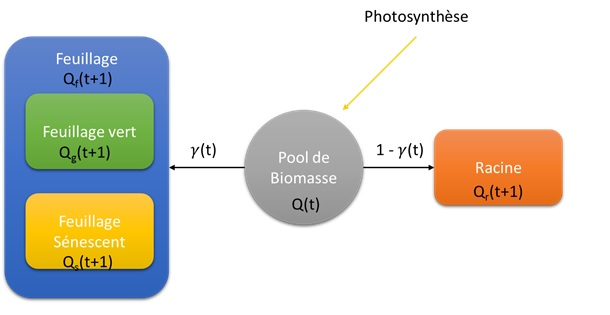
\includegraphics[scale=1.0]{./img/sBeetRoot.jpg}
   \caption{Schéma du modèle LNAS appliqué à la betterave}
   \label{fig:sBeetRoot}
   
   \end{center}
 \end{figure}
 
+Production de Biomasse :
 \[ \mathrm{Q}(t) = \big(\mu\cdot\mathrm{PAR}(t)(1-e^{-\lambda\mathrm{Q_g}(t)}\big)\cdot(1+\mathrm{\eta_Q}(t)) \]
 
+Allocation au feuillage :
 \[ \mathrm{Q_f}(t+1) = \mathrm{Q_f}(t) + \mathrm{\gamma}(t)\cdot\mathrm{Q}(t) \]
 
+Allocation à la racine :
 \[ \mathrm{Q_r}(t+1) = \mathrm{Q_r}(t) + (1 -\mathrm{\gamma}(t))\cdot\mathrm{Q}(t) \]
 
+Fonction d'allocation :
 \[ \mathrm{\gamma}(t) = (\gamma_0 + (\gamma_f - \gamma_0)\cdot\mathrm{G_a}(\mathrm{\tau}(t)))\cdot(1+\mathrm{\eta_{\gamma}}(t)) \]
 
+Fonction de sénescence :
 \[ \mathrm{Q_s}(t) = \mathrm{G_s}(\mathrm{\tau}(t)- \tau_{sen})\mathrm{Q_f}(t) \]
 
+Part de la biomasse produite qui arrive aux feuilles vertes :
 \[\mathrm{Q_g}(t) = \mathrm{Q_f}(t) - \mathrm{Q_s}(t) \]
 
 \begin{itemize}
 
 \item $\mathrm{Q}(t)$ : Production de biomasse au jour t par unité de surface.
 \item $\mu$ : Efficacité énergétique
 \item $1-e^{-\lambda\mathrm{Q_g}(t)}$ : Fraction des radiations interceptées
 \item $\mathrm{PAR}(t)$ : quantité de radiations photosynthétiquement actives par unité de surface.
 \item $\lambda$ : paramètre
 \item $\mathrm{Q_g}(t)$ : masse total des feuilles vertes au jour t
 \item $\mathrm{Q_f}(t)$ : masse total du feuillage au jour t
 \item $\mathrm{Q_s}(t)$ : masse total du feuillage sénescent au jour t 
 \item $\mathrm{\gamma_0}, \mathrm{\gamma_f}$ : paramètres
 \item $\mathrm{\eta}(t)$ : variables aléatoires normales 
 \item $\mathrm{G}(t)$ : variables aléatoires lognormales
 \item $\mathrm{\tau}(t)$ : temps thermique au jour t (température cumulée depuis l'émergence de la plante)
 \item $\tau_{sen}$ : temps thermique où la sénescence commence.
 \item Les paramètres des variables aléatoires font parti des paramètres du modèle.
 
 \end{itemize}